% DSA4212 project report: working draft, two-column layout.
% Source of truth: the team's Overleaf project; report-draft/main.tex mirrors it. Figures and results tables come from code/pipeline/make_report_assets.py.
% Status markers, all defined below and listed in REPORT_PLAN.md:
%   \resultpending{...}  text that waits for final scoring
%   \pendingfig{h}{...}  space reserved for a figure, table or text at its expected final size
%   \planned             analysis that has not been run yet; delete it if the analysis is dropped
%   \verify{...}         statement to re-check after the 10-seed baseline is scored
%   \needinfo{...}       details still to fill in, such as email addresses
% Set \draftmarksfalse for submission: any marker still in use then stops the build.

% The course template uses 12pt; 10pt is needed to meet the 10-page limit.
\documentclass[10pt,twocolumn]{article}

%%%%%%%%%%%%%%%%%%%%%%%%%%%%%%%%%%%%%%%%%%%%%%%%%%%%%%%%%%%%%%%%%%%%%%%%%%%%%%%%%%%%%%
% Course template preamble (unchanged)
\usepackage[numbers,sort]{natbib}
\usepackage{amsfonts, amsmath}
\usepackage{graphicx}
\usepackage{libertine}
\usepackage{fullpage}
\usepackage{hyperref}
\hypersetup{
    colorlinks = true,
    linkcolor = blue,
    urlcolor  = blue,
    citecolor = blue,
    anchorcolor = blue}
\urlstyle{same}
%%%%%%%%%%%%%%%%%%%%%%%%%%%%%%%%%%%%%%%%%%%%%%%%%%%%%%%%%%%%%%%%%%%%%%%%%%%%%%%%%%%%%%

% Additions for this report: tables, draft markers, compact lists
\usepackage{booktabs,tabularx,array}
\usepackage{xcolor}
\usepackage{enumitem}
\setlist{nosep,leftmargin=*}
\setlength{\bibsep}{1pt}
\setlength{\emergencystretch}{2em}
% Uniform spacing: no stretched gaps between paragraphs, and tighter headings and floats
\raggedbottom
\makeatletter
\renewcommand\section{\@startsection{section}{1}{\z@}{2.6ex \@plus .6ex \@minus .2ex}{1.4ex \@plus .2ex}{\normalfont\Large\bfseries}}
\renewcommand\subsection{\@startsection{subsection}{2}{\z@}{2.2ex \@plus .5ex \@minus .2ex}{1ex \@plus .2ex}{\normalfont\large\bfseries}}
\renewcommand\paragraph{\@startsection{paragraph}{4}{\z@}{1.4ex \@plus .4ex \@minus .2ex}{-1em}{\normalfont\normalsize\bfseries}}
\makeatother
\setlength{\textfloatsep}{12pt plus 2pt minus 2pt}
\setlength{\dbltextfloatsep}{12pt plus 2pt minus 2pt}
\setlength{\abovecaptionskip}{5pt}
\setlength{\columnsep}{0.25in}
% Two-column layout: narrower margins than fullpage's 1in, and more room for floats
\usepackage[margin=0.75in]{geometry}
\renewcommand{\dbltopfraction}{0.85}
\renewcommand{\dblfloatpagefraction}{0.8}
\renewcommand{\topfraction}{0.85}
\renewcommand{\textfraction}{0.1}
\setcounter{dbltopnumber}{3}

\newif\ifdraftmarks
\draftmarkstrue

\ifdraftmarks
  \newcommand{\resultpending}[1]{\par\smallskip\noindent\fcolorbox{orange}{orange!8}{\parbox{\dimexpr\linewidth-2\fboxsep-2\fboxrule}{\small\textbf{Results pending.} #1}}\par\smallskip}
  \newcommand{\pendingfig}[2]{\par\smallskip\noindent\fcolorbox{orange}{orange!8}{\parbox[c][#1]{\dimexpr\linewidth-2\fboxsep-2\fboxrule}{\centering\small #2}}\par\smallskip}
  \newcommand{\planned}{\textsuperscript{\textcolor{red}{[planned]}}}
  \newcommand{\verify}[1]{\textcolor{red}{\small [check after rescoring: #1]}}
  \newcommand{\needinfo}[1]{\textcolor{red}{[#1]}}
\else
  \newcommand{\resultpending}[1]{\errmessage{Unresolved results-pending marker}}
  \newcommand{\pendingfig}[2]{\errmessage{Unresolved figure marker}}
  \newcommand{\planned}{\errmessage{Unresolved planned marker}}
  \newcommand{\verify}[1]{\errmessage{Unresolved verify marker}}
  \newcommand{\needinfo}[1]{\errmessage{Unresolved information marker}}
\fi

\newcommand{\figw}{\linewidth}% width of the one-column figures
\newcommand{\figwide}{0.62\linewidth}% width of the page-wide figures
\newcommand{\ceil}[1]{\lceil #1 \rceil}
\newcommand{\Weib}{\mathrm{Weibull}}

\begin{document}

\makeatletter
\twocolumn[\begin{@twocolumnfalse}
\title{\vspace{-3.2em}\Large What LLM-Evolved Bin-Packing Rules Learn, and Why They Break: A Controlled Study under a Matched Evaluation Budget}
\date{\vspace{-3.4em}}
\maketitle
\vspace{-1.6em}

{\small\noindent{\bf Group Composition:} Lee Jia Kang, A0281521M, jiakanglee@u.nus.edu; Jin Syl Ngoh, A0271752A, jinsyl.ngoh@u.nus.edu; Chung Zhi Hao, Nicholas, A0249012N, nicholas.czh@u.nus.edu.\\{\bf Github Repository:} \url{https://github.com/jinsyl123/dsa4212-project}\par}
\vspace{-0.6em}

\begin{abstract}
\noindent Large language models (LLMs) embedded in evolutionary program search have produced online bin-packing heuristics that outperform Best Fit on their training distributions. We ask what determines where such rules succeed or fail when evolution is held to the same budget as parameter tuning. Using Evolution of Heuristics (EoH) with an inexpensive model and 300 program evaluations per run, we compare evolved rules with Best Fit and with a three-parameter Best Fit tuned under the same budget, on eleven held-out test sets that each alter the problem in one controlled way. Two ablations vary the packing convention and prompt, and the diversity of the training data, alongside a no-evolution control, with predictions recorded before scoring.
In distribution, evolved rules frequently beat Best Fit, and did so in all ten runs once the prompt stated the task and how bins are offered, but only 1 of 50 beat the tuned Best Fit of its setting. Tuned Best Fit, however, degraded severely on one distribution shift and modestly on others. In these runs the largest gains and the worst failures were associated with two behaviours: opening an empty bin while a used bin could hold the item, and constants fitted to the training item-to-bin ratio. Most collapsing rules matched Best Fit once they could choose only among used bins, and a controlled sweep of the ratio showed failure beginning near the threshold predicted from one rule's constants.
\end{abstract}
\vspace{0.4em}
\end{@twocolumnfalse}]
\makeatother

\section{Introduction}

In online bin packing, items arrive one at a time and each must be placed in a bin immediately, without knowing what comes next, so as to use as few bins as possible. The standard solutions are hand-designed rules such as Best Fit, which places each item in the fullest bin that can hold it, and First Fit, which uses the earliest such bin~\citep{sgall2014online}. Best Fit is simple and hard to beat: it ranked first overall in a comparison with published evolved rules across twelve datasets~\citep{sim2025beyond}.

A recent line of work has an LLM write the rule instead. FunSearch~\citep{romera2024funsearch} asks an LLM to propose a priority function that scores each bin for the current item, rates each proposal by packing training instances, and keeps and varies the best proposals in an evolutionary loop. Evolution of Heuristics (EoH)~\citep{liu2024eoh} builds on this by evolving a short natural-language description of each heuristic together with its code, requiring far fewer LLM queries. On Weibull instances with 5,000 items, FunSearch reports reducing the excess bins of Best Fit from 3.98\% to 0.68\%~\citep{romera2024funsearch}, and EoH reports matching FunSearch's heuristic on its own instances (0.80\% for both, against Best Fit's 4.08\%) with about 2,000 queries, against roughly a million for FunSearch~\citep{liu2024eoh}.

Two results in the literature shaped the question we set out to answer. Sim et al.~\cite{sim2025beyond} evaluated published evolved rules on twelve datasets and found that most did not generalise beyond their training distribution, so a gain on training-like data says little about where a rule remains useful or why it stops being so. Nakajima~\cite{nakajima2026soft} showed, in a study of packing congruent shapes, that a new method's apparent advantage over its baseline disappeared once the baseline received comparable tuning effort, and Best Fit receives no tuning at all. We therefore ask a single question:

\begin{quote}
\emph{What determines where LLM-evolved online bin-packing rules succeed or fail, when evolution is held to the same evaluation budget as parameter tuning?}
\end{quote}

We first establish where evolved rules win and lose on held-out data against Best Fit and a budget-matched tuned Best Fit. EoH and tuned Best Fit are two optimisers of the same training objective with the same number of evaluations: one searches over programs with an LLM, and the other searches the three integer parameters of a fixed rule at random. We then test candidate explanations through controlled changes to the search and by re-scoring the final programs under controlled conditions. We find that, in distribution, tuned Best Fit beats all but one of 50 evolved rules; that the largest gains and the worst failures of both come from one strategy, opening an empty bin while a used bin has room; and that telling the LLM how bins are offered made every seed beat Best Fit but also produced the worst failures, which a sweep traces to constants fitted to the training item-to-bin ratio. Section~\ref{sec:decisions} positions the study within the literature and justifies our main design choices.

\section{Related work and positioning}
\label{sec:decisions}

\paragraph{LLM-guided program search.} We retain FunSearch's restriction to a fixed skeleton and a single evolved function~\citep{romera2024funsearch} because it keeps feasibility checking and scoring outside the evolved code and yields programs short enough to interpret, as an explanatory question requires. ReEvo adds reflective prompting, at the expense of additional LLM calls per evaluated program, and its bin-packing experiments address the offline problem through ant colony heuristics~\citep{ye2024reevo}. We therefore take EoH's setup as our starting point, using the implementation in LLM4AD~\citep{liu2026llm4ad}, an open-source platform for such methods, and report each departure from it in Table~\ref{tab:eoh}. Ye et al.~\cite{ye2024reevo} also argue that such methods should be compared by the number of heuristic evaluations and not by LLM queries. We adopt that unit, since wall-clock time would penalise API latency and a parameter tuner incurs no LLM cost, and we allow every method 300 evaluations. This is about one seventh of EoH's 2,000 queries, so our conclusions concern a low-budget regime. As exploratory runs varied widely between seeds, we preferred many short searches to a few long ones: ten per ablation and control, and six for the baseline, later extended to ten (Section~\ref{sec:stats}).

\paragraph{Generalisation and comparators.} Reported gains are typically measured on the training distribution. Beyond the comparison of Sim et al.~\cite{sim2025beyond}, the EoH-S study~\cite{liu2025eohs} reports that published single rules perform worse than Best Fit, FunSearch's by about a factor of four, on a set spanning many Weibull shapes and scales. As these benchmarks vary many properties at once, they cannot identify which change causes a failure, and we therefore construct test sets that each alter one generator parameter. We generate our own capacity series, as the EoH repository reports that their capacity-500 experiments changed the capacity of only one of five instances~\citep{eohreadme2026}. The same source attributes a sharp divergence between two rules of equal training fitness to absolute-magnitude terms, which makes a set that rescales items together with the bin (\texttt{cap500\_scaled}) informative. A second concern is the comparator. Best Fit has no parameters and receives no search budget, so beating it cannot separate the contribution of the LLM from that of optimising anything at all against the training set, the concern that Nakajima's result raises (Section~1). We therefore add a variant of Best Fit tuned under the same 300 evaluations, whose form follows the strategy FunSearch reports for several of its discovered heuristics, avoiding small gaps that are unlikely ever to be filled~\citep{romera2024funsearch}. This differs from the tuning study of Sim et al.~\cite{sim2025beyond}, who adjusted the constants of published evolved rules and found that doing so did not repair their lack of generality.

\paragraph{The roles of search, model and problem information.} Zhang et al.~\cite{zhang2024eps} and the LLM4AD study~\cite{liu2026llm4ad} find that evolutionary search generally outperforms repeated sampling from an LLM, although not on every task, at budgets of 10,000 and 2,000 evaluations respectively. This need not hold at 300 evaluations, so we include a no-evolution control. Both studies also find that larger or code-specialised models are not reliably better, which motivates fixing one inexpensive model and spending the budget on repeated searches. The value of additional information is less settled. BLADE~\citep{vanstein2025blade} identifies the exploitation of problem information as a capability worth testing but does not itself run such an ablation, and LLM4AD's default prompt does not state what its bin array contains; Ablation~1 (Section~\ref{sec:settings}) varies this information. EoH-S~\citep{liu2025eohs} trains on many Weibull shapes and scales, but its strongest results are for sets of rules scored by the best rule per instance, which presumes that the best rule for each instance is known in advance. We keep a single rule and ask only whether more varied training data prevents failures, which is the subject of Ablation~2 (Section~\ref{sec:settings}).

\section{Problem formulation}
\label{sec:formulation}

An instance consists of integer item sizes $s_1,\dots,s_n$ and a capacity $C$. A \emph{priority rule} $h$ receives the current item $s$ and the vector $r$ of remaining capacities of the bins into which it fits, and returns one score per bin. The item is placed irrevocably in the highest-scoring bin, with ties resolved in favour of the earliest. The rule is never told the capacity.

Under the \emph{pre-allocated} convention (\texttt{funsearch} mode in the repository), used by FunSearch, EoH and LLM4AD and retained here so that our packings are comparable with theirs, $n$ empty bins exist from the start and are offered alongside used bins. Because an empty bin is always offered, $\max_j r_j = C$, so a rule can infer the capacity indirectly. Under the \emph{AnyFit} convention~\citep{sgall2014online}, $h$ scores only used bins and a new bin opens only when none fits, so restricting search to this class removes the option of opening a new bin while a used one has room. Best Fit and First Fit pack identically under both. A placement is \emph{fresh} if it opens an empty bin while a used bin had room, and the \emph{fresh-bin rate} $\phi$ is the share of fresh placements among those where a used bin had room.

Quality is the relative excess over a lower bound, $(\text{bins}-\mathrm{LB})/\mathrm{LB}$, averaged over instances. The continuous bound is $L_1=\ceil{\sum_i s_i/C}$. The Martello--Toth bound $L_2$~\citep[\S8.3.2]{martello1990knapsack} also accounts for items larger than half a bin, which cannot share one, and for how far smaller items can fill the space they leave. The FunSearch paper reports excess over $L_2$, whereas its released code~\citep{funsearchcode}, like that of EoH~\citep{eohreadme2026}, computes $L_1$. We use $L_1$ during search and report $L_2$, because $L_1$ is loose when many items exceed half a bin, as on our \texttt{scale65} set, where about 63\% do. The two bounds coincide on all our test sets except \texttt{scale65} and the control set.

\section{Experimental design}
\label{sec:design}

\subsection{Search and evaluation}
Each run executes EoH in LLM4AD~\citep{liu2026llm4ad} (commit \texttt{73ae214}) with the settings in Table~\ref{tab:eoh}, starting from LLM4AD's template, whose body is Best Fit. The prompts are LLM4AD's except where a setting changes them (Section~\ref{sec:settings}), with one addition applied identically everywhere: formatting instructions that reduce unparseable replies. LLM4AD describes the input only as an ``array of capacities for each bin'', without stating that these are remaining capacities or that empty bins are included. We keep this wording for comparability, although it may encourage rules that open new bins. LLM4AD discards as a duplicate any candidate whose code or score equals that of a population member. LLM sampling is unseeded and EoH runs two samplers in parallel, so a search cannot be repeated exactly. We refer to each independent search as a \emph{seed}, report the spread over seeds and publish every run's programs, scores and logs.

\begin{table*}[t]
\centering\footnotesize
\caption{Our setup relative to the EoH paper's online bin-packing experiment~\citep{liu2024eoh}. Selection (best on training) and the skeleton (a priority function, with empty bins offered) are kept.}
\label{tab:eoh}
\begin{tabularx}{\linewidth}{@{}lp{0.2\linewidth}p{0.24\linewidth}X@{}}
\toprule
Element & EoH paper & This study & Reason\\
\midrule
Budget & 2,000 LLM queries & 300 evaluations & Ten seeds per ablation and control, six for the baseline (later ten), within a fixed LLM budget\\
Model & GPT-3.5-turbo & Gemini 3.5 Flash Lite via OpenRouter, low reasoning effort & Inexpensive; larger models are not reliably better~\citep{zhang2024eps,liu2026llm4ad}\\
Population & 20 & 10 & LLM4AD's recommended size at this budget\\
Operators & E1, E2, M1, M2, M3 & E1, E2, M1, M2 & LLM4AD does not implement M3 (code, commit 73ae214)\\
Training set & 5 instances of 5,000 items & 32 instances of 200--2,000 items & Instance-size range of EoH-S~\citep{liu2025eohs}\\
Fitness & Mean $\mathrm{lb}/n$ & Minus mean excess over $L_1$ & Relative gap, as in EoH-S~\citep{liu2025eohs}; counts instances of different sizes and capacities equally\\
\bottomrule
\end{tabularx}
\end{table*}

Following the principle of method-independent logging in BLADE~\citep{vanstein2025blade}, one evaluator scores all candidates and records every program, token count and cost, together with every prompt and response for all runs except baseline seeds 0--5, which predate that logging. Programs run in a separate process with a time limit of 60\,s per evaluation during search and 900\,s per held-out set. A final program that fails on an instance receives the excess of Next Fit, which keeps only the most recent bin open, so that failures cannot flatter a mean, although a rule could in principle perform worse than Next Fit. Static checks flag non-deterministic or state-reading code without removing it. They can be circumvented, so best programs are also re-scored repeatedly and under shuffled instance order, which exposes randomness or carried state only if a bin count changes.

\subsection{Instance sets}
Table~\ref{tab:sets} lists the sets, frozen before the ablations were scored. Search sees only its training set, and the validation set is used only to select one seed per setting for Table~\ref{tab:cost}; no run is discarded. Each test set departs in one stated way from \texttt{id\_5k}, which itself differs from training only in the number of items, except for two deliberate cases: \texttt{cap500\_scaled} changes units while preserving the item-to-bin ratio, and \texttt{uniform} is generated like OR-Library's binpack1--4 at 1,000 items, as described in~\citep{romera2024funsearch}, without using the original files. On the control set every rule must use one bin per item.

\begin{table*}[t]
\centering\footnotesize
\caption{Instance sets. Weibull sizes follow~\citep{romera2024funsearch}, rounded and clipped to $[1,C]$; $\bar s/C$ is the approximate mean item size relative to capacity. Test sets contain 10 instances each, since with 5 a rule that wins on all of them still cannot reach $p<0.05$ in the sign test; their names omit the \texttt{test\_} prefix used in the repository.}
\label{tab:sets}
\setlength{\tabcolsep}{3pt}
\begin{tabular}{@{}llrrll@{}}
\toprule
Role / what changes & Set & Items & $C$ & Item sizes & $\bar s/C$\\
\midrule
Search & \texttt{train} (32 instances) & 200--2,000 & 100 & $\Weib$(shape 3, scale 45) & 0.40\\
Search (A2a) & \texttt{train\_mixed} (32) & 200--2,000 & 100 & shapes 2 and 4, scale 45 & 0.40\\
Search (A2b) & \texttt{train\_mixed\_cap} (32) & 200--2,000 & 100, 300 & shape 3, scale 45 & 0.40, 0.13\\
Selection only & \texttt{val} (10) & 1,000 & 100 & as \texttt{train} & 0.40\\
\midrule
In distribution & \texttt{id\_5k} & 5,000 & 100 & as \texttt{train} & 0.40\\
Number of items & \texttt{size\_1k}, \texttt{size\_10k} & 1,000; 10,000 & 100 & as \texttt{train} & 0.40\\
Capacity & \texttt{cap200}, \texttt{cap500} & 5,000 & 200; 500 & as \texttt{train} & 0.20; 0.08\\
Units & \texttt{cap500\_scaled} & 5,000 & 500 & shape 3, scale 225 & 0.40\\
Item-to-bin ratio & \texttt{scale25}, \texttt{scale65} & 5,000 & 100 & shape 3, scale 25; 65 & 0.22; 0.58\\
Spread of sizes & \texttt{shape\_k1.5}, \texttt{shape\_k5} & 5,000 & 100 & shape 1.5; 5, scale 45 & 0.40; 0.41\\
OR-Library style & \texttt{uniform} & 1,000 & 150 & Uniform$[20,100]$ & 0.40\\
Scoring check & \texttt{control} & 1,000 & 100 & Uniform$[51,100]$ & 0.76\\
\bottomrule
\end{tabular}
\end{table*}

\subsection{Comparators}
\label{sec:comparators}
The classical comparator is Best Fit, as benchmarked in~\citep{sim2025beyond}, whereas evolved rules and tuned Best Fit are scored under the convention of their setting (AnyFit in A1a, pre-allocated elsewhere). Any score strictly decreasing in the post-placement gap $g=r-s$ packs exactly as Best Fit does, so a rule that behaves differently must not be strictly decreasing in $g$. We use one of the simplest such forms, a penalty on a range of gaps, which matches the strategy FunSearch reports for several of its heuristics (Section~\ref{sec:decisions}). \emph{Tuned Best Fit} is
\[
h_{\ell,u,p}(s,r) \;=\; -g \;-\; p\cdot\mathbf{1}\{\ell<g<u\}, \qquad g=r-s,
\]
with integers $\ell\in[0,10]$, $u\in[\ell+2,40]$ and $p\in[1,100]$, in item units. Random search scores Best Fit and then 299 distinct parameter triples per seed on the training set, drawn from a seeded generator so that the tuner is exactly reproducible, and is repeated for each experiment's training set and packing convention. Random search is the simplest tuner, so its result is a floor for what tuning this rule can achieve, and we did not use a model-based method such as Bayesian optimisation. One seed's 299 triples cover 0.8\% of the 37,400 in the space, but a longer search would change little: in the baseline, the ten seeds together score 2,881 distinct triples besides Best Fit, and the best of them, at 2.36\% training excess, is only 0.05\,pp below the median seed's 2.41\%.

\subsection{Sequence of controlled comparisons}
\label{sec:settings}
Table~\ref{tab:settings} lists the settings in the order they were designed. The model, the budget, the test sets and the scoring are the same throughout, with ten seeds per ablation and control and six for the baseline, later extended to ten (Section~\ref{sec:stats}). Each setting changes one element relative to its comparison row, except the control, whose method also changes the prompt, and A1b, whose prompt change has two parts. Only A1a searches under the AnyFit convention; every other setting is pre-allocated.

The settings were designed in stages, each prompted by the results of the previous one (last column). Ablation~2 was planned provisionally as mixed-shape training and was finalised, with A2b added, only after Ablation~1 was scored (Section~\ref{sec:a2}). Stage~4 tests the resulting explanations on the final programs, with no further search.

\begin{table*}[t]
\centering\footnotesize
\caption{Experimental settings in the order they were designed. Everything not listed under ``Change'' is held fixed.}
\label{tab:settings}
\begin{tabularx}{\linewidth}{@{}clp{0.3\linewidth}lX@{}}
\toprule
Stage & Setting & Change & Compared with & Prompted by\\
\midrule
1 & Baseline & None: EoH, default prompt, pre-allocated convention, \texttt{train} & Best Fit, tuned Best Fit & The research question\\
2 & A1a & Search under the AnyFit convention & Baseline & Stage 1: gains and a failure came from fresh bins\\
2 & A1b & Prompt states the task and how bins are offered; empty bins still offered & Baseline & Stage 1: default prompt does not say what the bin array holds\\
2 & Control & LLM4AD RandSample: no evolution and a fixed prompt & Baseline & Stage 1: do the gains need evolution at this budget?\\
3 & A2a & Training on mixed shapes & Baseline & Stage 1 shape failures; kept after Stage 2\\
3 & A2b & A1b, training on mixed capacities & A1b & Stage 2: A1b's collapses on small relative item sizes\\
4 & Re-scoring & Final programs without access to empty bins; ratio and capacity sweeps & Same programs, empty bins offered & Stages 1--3: explanations to test\\
\bottomrule
\end{tabularx}
\end{table*}

\subsection{Measurement and pre-specified predictions}
\label{sec:stats}
For every setting we report excess over $L_2$ on all held-out sets; running time per instance and failed instances for the \emph{use} of a rule; and LLM cost, tokens, the proportion of valid programs and the number of unique programs for its \emph{discovery}.

Comparisons with a reference (Best Fit, or tuned Best Fit averaged per instance over its seeds) are paired by instance. For each seed and set we compute a 95\% bootstrap interval of the mean paired difference (10,000 resamples) and a two-sided exact sign test. A rule is \emph{better} or \emph{worse} only if the interval excludes zero and $p<0.05$, a \emph{tie} if identical on every instance, and otherwise \emph{unclear}. With ten instances this requires at least nine wins when all ten differ, and because tied instances are uninformative, no verdict of better or worse is possible with five or more ties. \emph{Unclear} therefore usually denotes a small or inconsistent effect and not the absence of one. Tables give the numbers of seeds that are better and worse as better/worse; the others tie or are unclear. Because tuned Best Fit yields one program per seed, the averaged reference compares each evolved rule with the average tuned run and not with a single packing. Seed counts between settings are compared by a two-sided Fisher exact test. A \emph{fresh-bin seed} has $\phi>0.01$ on the training set, and a \emph{collapse} is a mean excess more than 100 percentage points above Best Fit. We apply no correction for multiple comparisons, since with ten instances and ten seeds few of these tests could pass one, so $p$-values and single verdicts are descriptive and claims rest on patterns repeated across seeds and sets.

Because each stage was designed from the previous one's results, we guard against selective reporting: predictions and the conclusion to be drawn from each outcome were recorded before the corresponding results were scored, the test sets were frozen in advance, and anything decided after scoring is labelled exploratory. The principal predictions are reported with their outcomes in Table~\ref{tab:pred1}, and the full list is in \texttt{code/docs/claims.md}. Predictions for the secondary A1 sets were added after scoring and do not count as confirmations, and A1b's collapses were found after scoring. The baseline was run for six seeds and later extended to ten; seeds 6--9 and the robustness rule below were added after Ablation~1 and the control were scored. Comparisons against the six originally planned seeds remain primary, with ten-seed comparisons alongside, and a seed-count result significant against only one of the two is called \emph{not robust}. Explanatory analyses are described where they are used in Section~\ref{sec:results}, and those that post-date the frozen predictions are exploratory.

\section{Results and analysis}
\label{sec:results}

\subsection{Where evolved rules succeed and fail}
\label{sec:res-baseline}
We begin with the baseline of Stage~1, asking where evolved rules win and lose at low budget; later stages are reported where they are introduced.

\begin{table*}[t]
\centering\footnotesize
\caption{Stage~1. Mean excess over $L_2$ (\%) and per-seed verdicts against each reference, written better/worse: the number of the 10 seeds that are better and worse; the others tie or are unclear. Verdicts are defined in Section~\ref{sec:stats}. Counts use all ten baseline seeds, including seeds 6--9 added after Ablation~1 and the control were scored; the text gives the six-seed counts and a caveat on \texttt{scale25}. Columns: \texttt{id\_5k}, \texttt{size\_1k}, \texttt{size\_10k}, \texttt{cap200}, \texttt{cap500}, \texttt{cap500\_scaled}, \texttt{scale25}, \texttt{scale65}, \texttt{shape\_k1.5}, \texttt{shape\_k5}, \texttt{uniform}.}
\label{tab:baseline}
% Generated by code/pipeline/make_report_assets.py; do not edit by hand, rerun the script.
% Sources, under code/results/: excess means from <setting>/final_summary.csv for the baseline (Best Fit's row from
% the baseline's final_per_instance.csv); better/worse verdict counts from <setting>/paired_stats.csv.
\footnotesize\setlength{\tabcolsep}{3.5pt}\begin{tabular}{@{}lrrrrrrrrrrr@{}}
\toprule
 & \texttt{id\_5k} & 1k & 10k & c200 & c500 & c500s & s25 & s65 & k1.5 & k5 & unif. \\
\midrule
Best Fit, excess \% & 4.08 & 4.44 & 3.99 & 1.52 & 0.52 & 4.38 & 1.68 & 0.43 & 1.35 & 8.32 & 5.08 \\
Tuned Best Fit, excess \% & 1.60 & 2.21 & 1.34 & 1.46 & 0.50 & 5.19 & 3.79 & 0.40 & 2.45 & 30.36 & 3.17 \\
\quad better/worse than Best Fit & 10/0 & 10/0 & 10/0 & 4/0 & 0/0 & 0/10 & 3/4 & 0/0 & 3/7 & 0/10 & 10/0 \\
Baseline, excess \% & 3.79 & 4.27 & 3.73 & 1.55 & 0.54 & 4.16 & 1.79 & 0.47 & 1.57 & 8.62 & 4.63 \\
\quad better/worse than Best Fit & 5/0 & 2/0 & 5/0 & 0/1 & 0/1 & 3/1 & 0/1 & 0/1 & 3/1 & 1/2 & 4/0 \\
\quad better/worse than tuned & 0/10 & 0/10 & 0/10 & 0/1 & 0/1 & 10/0 & 10/0 & 0/1 & 9/1 & 10/0 & 0/10 \\
\bottomrule
\end{tabular}

\end{table*}

In distribution, half of the evolved rules beat Best Fit (Table~\ref{tab:baseline}): 5 of 10 seeds are better on \texttt{id\_5k} (3 of the original 6) and none is worse. Seeds that are neither better nor worse either pack exactly as Best Fit does or differ too little to satisfy the verdict rule; on \texttt{cap200}, \texttt{cap500}, \texttt{scale25} and \texttt{scale65}, the unclear seeds differ from Best Fit by at most about 0.05\,pp. The gains are uneven, 1.20\,pp for seeds 4 and 5 and about 0.2\,pp for seeds 2, 8 and 9. First Fit is no better than Best Fit on any set, so Best Fit is the classical comparator throughout. The budget-matched reference changes this picture. Tuned Best Fit is better than Best Fit in all ten seeds, by 2.48\,pp on average, and every evolved rule is worse than it on \texttt{id\_5k}, both size sets and \texttt{uniform}.

On three of the shifted sets the ranking reverses. Tuned Best Fit is worse than Best Fit on \texttt{cap500\_scaled} and \texttt{shape\_k5} in all ten seeds and on \texttt{shape\_k1.5} in seven, reaching 30.36\% on \texttt{shape\_k5} against Best Fit's 8.32\%. All ten evolved seeds are better than it on \texttt{cap500\_scaled} and \texttt{shape\_k5}, and nine on \texttt{shape\_k1.5}, and at most 2 of 10 are worse than Best Fit on any set. All ten are also better on \texttt{scale25}, but there the averaged reference is raised by two tuned seeds (5.78\% and 17.46\%, against 1.47--2.33\% for the other eight); against the six originally planned tuned seeds, 2 of 6 evolved seeds are better, 3 unclear and 1 worse. The verdicts against tuned Best Fit on this set in Tables~\ref{tab:a1} and~\ref{tab:a2} carry the same caveat. The six original seeds otherwise give the same picture: on \texttt{id\_5k} 3 are better than Best Fit, 2 tie and 1 is unclear, and all 6 are worse than tuned Best Fit. On \texttt{cap200}, \texttt{cap500} and \texttt{scale65} the mean excesses of evolved rules and tuned Best Fit differ by less than 0.1\,pp. Beating Best Fit is therefore a weak test at this budget: a three-parameter search achieves more in distribution, and the two kinds of rule are separated mainly by their behaviour under shift.

\begin{figure}[t]% onecolumn
\centering
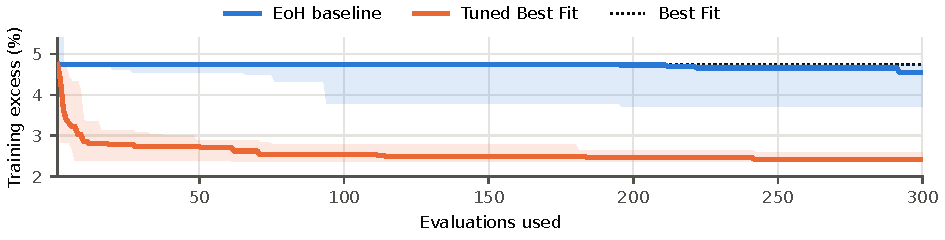
\includegraphics[width=\figw]{figures/convergence.pdf}
\caption{Best training excess found so far against evaluations used, in the baseline. Lines show the median of ten seeds and shaded areas the range across seeds. Training data only.}
\label{fig:convergence}
\end{figure}

Figure~\ref{fig:convergence} shows how the two searches use the budget on the training set. Tuned Best Fit's median reaches 2.86\% within 10 evaluations and ends at 2.41\%. EoH's median remains at Best Fit's 4.75\% until evaluation 186 and ends at 4.55\%, while its best seed reaches 3.72\%. EoH is still improving at evaluation 300, so a larger budget might narrow the gap.

\subsection{What the evolved rules do}
\label{sec:res-rules}
The seeds differ sharply in behaviour, so we examine each rule and re-score every final program under both packing conventions. Seeds 3, 4 and 5 are fresh-bin seeds and none of seeds 6--9 is, so the rate of 3 in 6 in the first runs fell to 3 in 10.

\begin{figure*}[t]
\centering
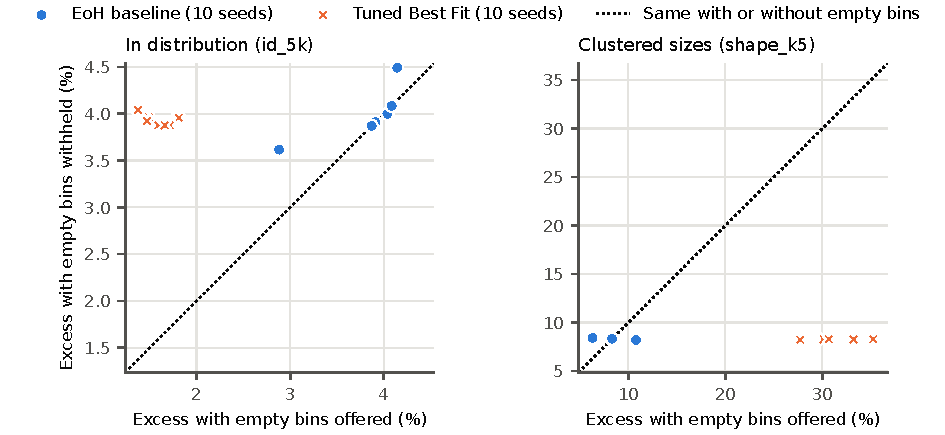
\includegraphics[width=\figwide]{figures/empty_bins.pdf}
\caption{Excess over the lower bound in the baseline with empty bins offered and withheld, one point per seed; identical rules coincide, so fewer than ten points are visible. On the dotted diagonal the excess is the same with or without empty bins; points above it were helped by empty bins and points below it were harmed.}
\label{fig:empty}
\end{figure*}

The largest gains we observed coincide with the \emph{fresh-bin strategy}, by which we mean opening fresh bins by design: every evolved rule that gained more than 1\,pp on \texttt{id\_5k} has $\phi>0.1$, although A1a and its tuned Best Fit (Section~\ref{sec:a1}) gain up to 0.93\,pp and 1.07\,pp without it. Seeds 4 and 5 are one rule written in two ways, $-x-\sin(\pi x)$ with $x=g/s$, and give identical packings. For items near the training mean (about 35--50 units), the rule opens an empty bin rather than leaving a gap of up to about one item, but it accepts near-exact fits; much smaller and larger items rarely trigger it. We interpret the strategy as succeeding when later small items fill the gaps, gaining 1.20\,pp on \texttt{id\_5k}, but not when sizes cluster in that band: on \texttt{shape\_k5} $\phi$ rises from 0.26 to 0.45 and the rule loses 2.49\,pp. Tuned Best Fit arrives at the same strategy with no LLM, at $\phi=0.33$ on \texttt{id\_5k} and $0.54$ on \texttt{shape\_k5}. Its ten seeds select nearly the same parameters, a penalty of 64--97 on leaving a gap strictly between 3--4 and 29--34 units. These thresholds are in item units, so at capacity 500 they cover gaps of less than 7\% of the bin, against up to 34\% at capacity 100, which is the mechanism we give for its loss on \texttt{cap500\_scaled} (Table~\ref{tab:attribution}).

Figure~\ref{fig:empty} separates what the strategy contributes. Most baseline seeds lie on the diagonal, so they do not depend on empty bins. With empty bins withheld, seeds 4 and 5 retain 0.47 of their 1.20\,pp in distribution and tuned Best Fit retains 0.16 of its 2.48\,pp, while on \texttt{shape\_k5} the excess falls to 8.19\% and 8.25\%, below Best Fit. The strategy therefore accounts both for its failure on clustered sizes and for most of the gain of parameters tuned with empty bins available; retuned under AnyFit, tuned Best Fit still gains 0.91\,pp (Section~\ref{sec:a1}). Across settings, the loss on \texttt{shape\_k5} rises with how often a rule opens fresh bins there (Figure~\ref{fig:phi}). Among rules with $\phi>0.1$ on that set, those below $\phi=0.44$ gain or break even, with one exception (A2a seed 6, 0.62\,pp worse at $\phi=0.34$); those at 0.44--0.45 lose 0.2--2.5\,pp; and every rule above 0.5 loses at least 19\,pp. This reading was made after scoring and is exploratory. Seed 3's loss on \texttt{shape\_k1.5} has another cause: it remains at 3.99\% without empty bins. Its score is a Gaussian so narrow that it underflows to zero for almost every bin, so ties reduce the rule to First Fit, except that it avoids any bin the item would fill to about 70\% of its remaining space.

\begin{figure}[t]% onecolumn
\centering
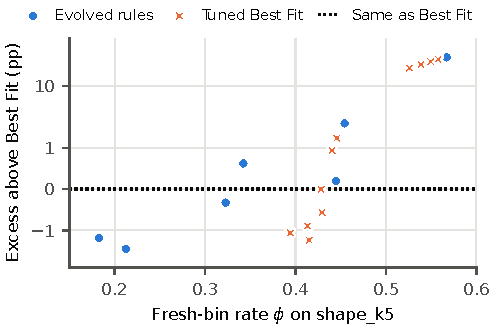
\includegraphics[width=\figw]{figures/fresh_rate.pdf}
\caption{Loss on clustered sizes against the fresh-bin rate $\phi$ on the same set, \texttt{shape\_k5}, for every rule with $\phi>0.1$ there: evolved rules of all settings and the tuned Best Fit seeds of the baseline, A2a and A2b; tuned seeds often select identical parameters, so many points coincide. The vertical axis is symmetric-logarithmic. Exploratory.}
\label{fig:phi}
\end{figure}

\subsection{Is the empty-bin option, the prompt or the search responsible?}
\label{sec:a1}
Stage~2 follows directly from that observation. If fresh-bin placements carry both the gains and the failures, removing the option or telling the LLM about it should change both. In A1a the fresh-bin behaviour is impossible by construction, so we ask whether EoH can still improve on Best Fit. In A1b the prompt states the task and explains that the scored bins are remaining capacities that include empty bins, so we ask whether informing the LLM makes the behaviour more frequent or earlier; because framing and bin description change together, any effect is attributed to the combination. The control asks whether evolution adds to repeated sampling at this budget, and retains the best of 300 samples from a fixed FunSearch-style prompt that shows Best Fit. We describe it as RandSample and not as EoH without search.

\begin{table*}[t]
\centering\footnotesize
\caption{Stage~2, in the format of Table~\ref{tab:baseline}. A1a's references are searched and scored under AnyFit. Verdicts against tuned Best Fit on \texttt{scale25} carry the caveat of Section~\ref{sec:res-baseline}. A1b's large means on \texttt{cap200}, \texttt{cap500} and \texttt{scale25} reflect the collapses of Section~\ref{sec:a2}.}
\label{tab:a1}
% Generated by code/pipeline/make_report_assets.py; do not edit by hand, rerun the script.
% Sources, under code/results/: excess means from <setting>/final_summary.csv for A1a, A1b and the control (Best Fit's row from
% the baseline's final_per_instance.csv); better/worse verdict counts from <setting>/paired_stats.csv.
\footnotesize\setlength{\tabcolsep}{3.5pt}\begin{tabular}{@{}lrrrrrrrrrrr@{}}
\toprule
 & \texttt{id\_5k} & 1k & 10k & c200 & c500 & c500s & s25 & s65 & k1.5 & k5 & unif. \\
\midrule
A1a, excess \% & 3.73 & 4.22 & 3.66 & 1.41 & 0.50 & 4.20 & 1.50 & 0.60 & 1.18 & 8.30 & 4.23 \\
\quad better/worse than Best Fit & 6/0 & 4/0 & 6/0 & 5/2 & 2/1 & 5/1 & 4/0 & 0/4 & 5/1 & 1/1 & 7/0 \\
\quad better/worse than tuned & 0/8 & 0/6 & 0/8 & 3/5 & 2/2 & 10/0 & 3/6 & 7/1 & 2/8 & 0/6 & 5/3 \\
Tuned, AnyFit, excess \% & 3.17 & 3.81 & 3.15 & 1.37 & 0.49 & 5.20 & 1.48 & 0.47 & 0.98 & 8.12 & 4.53 \\
A1b, excess \% & 3.53 & 4.05 & 3.44 & 138 & 571 & 6.35 & 95.14 & 0.43 & 1.29 & 8.21 & 4.41 \\
\quad better/worse than Best Fit & 10/0 & 3/0 & 9/0 & 0/5 & 0/5 & 5/1 & 1/5 & 0/0 & 2/0 & 2/1 & 4/0 \\
\quad better/worse than tuned & 0/10 & 0/9 & 0/10 & 0/6 & 0/5 & 9/1 & 6/4 & 0/0 & 10/0 & 10/0 & 1/8 \\
Control, excess \% & 4.08 & 4.44 & 3.99 & 1.52 & 0.52 & 4.38 & 1.68 & 0.43 & 1.35 & 8.32 & 5.08 \\
\quad better/worse than Best Fit & 0/0 & 0/0 & 0/0 & 0/0 & 0/0 & 0/0 & 0/0 & 0/0 & 0/0 & 0/0 & 0/0 \\
\quad better/worse than tuned & 0/10 & 0/10 & 0/10 & 0/0 & 0/0 & 10/0 & 10/0 & 0/0 & 10/0 & 10/0 & 0/10 \\
\bottomrule
\end{tabular}

\end{table*}

\paragraph{Removing the option (A1a).} Six of ten seeds are better than Best Fit on \texttt{id\_5k}, by up to 0.93\,pp with no fresh bins (Table~\ref{tab:a1}), so part of the gain does not depend on the fresh-bin strategy. The comparator changed the conclusion: searched under AnyFit, tuned Best Fit reaches 3.17\%, which is 0.91\,pp better than Best Fit against our prediction of 0.1\,pp, and it is better than 8 of the 10 A1a seeds. These rules also depend on their convention. If empty bins are offered again, the four best (seeds 1, 3, 6 and 7) open them in 64--73\% of choices and reach 60--82\% excess.

\paragraph{Informing the LLM (A1b).} All ten seeds are better than Best Fit on \texttt{id\_5k}, against 3 of 6 ($p=0.036$) and 5 of 10 ($p=0.033$), the only increase in seeds beating Best Fit with $p<0.05$ against both baselines. Seed 1 reaches 1.77\%, the closest of any evolved rule to tuned Best Fit's 1.60\%. The improvement did not arise as we predicted (Table~\ref{tab:pred1}): fresh-bin seeds reach only 6 of 10, short of the at least 8 we predicted, against 3 of 6 and 3 of 10 in the baseline, and there is no clear change in when the best rule is found. What did change is how rules use the capacity. Six of the ten final programs read it from the largest bin, against none in the baseline, A1a or A2a, and five of those six collapse on \texttt{cap500}. A1b's best rule, seed 1, does not read it: its denominator simplifies to $2s$ instead of the capacity, giving $-|g/(2s)-0.5|+1.5/g$.

\paragraph{No evolution (control).} All ten seeds end at exactly Best Fit, found at the first evaluation and never beaten, from about 30 unique programs of 300 against EoH's 207. No seed is better than Best Fit on \texttt{id\_5k}, against 3 of 6 ($p=0.036$) and 5 of 10 ($p=0.033$). The absence of fresh-bin seeds is not robust ($p=0.036$ and $0.21$). This is consistent with evolution contributing at this budget, although the control also uses a different prompt, so the two effects cannot be separated.

\begin{table*}[t]
\centering\footnotesize
\caption{Principal predictions with their outcomes. Stage~2 predictions (A1a, A1b, control) were recorded before scoring; Stage~3 predictions (A2a, A2b) after Stage~2 was scored and before any A2 run.}
\label{tab:pred1}
\begin{tabularx}{\linewidth}{@{}lXX@{}}
\toprule
Setting & Prediction & Outcome\\
\midrule
A1a & At least 4 of 10 seeds better than Best Fit on \texttt{id\_5k} & Held: 6 of 10\\
A1a & No seed worse on \texttt{shape\_k5} & Failed: seed 5 worse by 0.21\,pp\\
A1a & Tuned under AnyFit within 0.1\,pp of Best Fit & Failed: 0.91\,pp better\\
A1b & At least 8 of 10 fresh-bin seeds, with the best rule found earlier & Failed: 6 of 10. Discovery time, defined after scoring as the evaluation of the final rule: median 217 against about 200 expected (fresh-bin seeds: 192 in A1b against 212), so no clear change\\
A1b & More seeds better on \texttt{id\_5k}, more worse on \texttt{shape\_k5} & Held: 10 of 10. Failed: 1 worse\\
A1b & None made (found after scoring) & 5 of 10 collapse on \texttt{cap500}\\
Control & Most seeds at or near Best Fit; at most 2 of 10 fresh-bin seeds & Held: all 10 exactly Best Fit; 0 of 10\\
\midrule
A2a & At most 3 of 10 seeds worse on a shape set & Held: 1 ($p=0.12$ and $0.58$)\\
A2a & Smaller in-distribution gains, at most 5 of 10 better & Failed: 9 of 10; mean gain 0.44\,pp against 0.42\,pp (six seeds) and 0.30\,pp (ten seeds)\\
A2a & Lower fresh-bin rate & Direction held: 2 of 10 against 3 of 6 ($p=0.30$)\\
A2b & No collapses on \texttt{cap200} or \texttt{scale25} & Held: 0 against 4 of 10 ($p=0.087$)\\
A2b & At most 2 of 10 collapse on \texttt{cap500} & Held: 2 against 5 of 10 ($p=0.35$)\\
A2b & Smaller gain at capacity 100 & Held: 0.35\,pp against 0.56\,pp\\
\bottomrule
\end{tabularx}
\end{table*}

\subsection{Do failures originate in the training data?}
\label{sec:a2}
The results of Ablation~1 changed what Stage~3 needed to test. A1b's rules collapsed where items are small relative to the bin: 5 of 10 seeds on \texttt{cap500} and 4 of 10 on each of \texttt{cap200} and \texttt{scale25}, the last of which keeps the training capacity. None collapsed on \texttt{cap500\_scaled}, which has capacity 500 but the training ratio. This suggests that the failure follows the item-to-bin ratio and not the capacity itself, a pattern we identified after scoring and therefore treat as exploratory. No baseline seed collapses. Both A2 settings were fixed before any A2 run and ask whether failures come from training on a single condition; A2a's training shapes, 2 and 4, make the test shapes 1.5 and 5 an extrapolation. Best Fit's excess is much smaller at capacity 300, so selection is dominated by the capacity-100 half unless a rule fails outright. A2b can thus show whether diversity prevents the failure, but probably not whether rules learn to read capacity, and given A1b's collapse counts only \texttt{cap500} can reach significance under our seed-count test. Because mean excess is unbounded, unlike EoH's $\mathrm{lb}/n$, a collapsing rule is heavily penalised during search, which is partly a property of this objective.

\begin{table*}[t]
\centering\footnotesize
\caption{Stage~3, in the format of Table~\ref{tab:baseline}. Each setting's tuned Best Fit is retuned on its training set. A2b's large mean on \texttt{cap500} reflects two collapsing seeds, and its verdicts against tuned Best Fit on \texttt{scale25} carry the caveat of Section~\ref{sec:res-baseline}.}
\label{tab:a2}
\scriptsize\setlength{\tabcolsep}{2.5pt}\begin{tabular}{@{}lrrrrrrrrrrr@{}}
\toprule
 & \texttt{id\_5k} & 1k & 10k & c200 & c500 & c500s & s25 & s65 & k1.5 & k5 & unif. \\
\midrule
A2a, excess \% & 3.64 & 4.21 & 3.60 & 1.44 & 0.50 & 4.16 & 1.56 & 0.50 & 1.25 & 8.43 & 4.53 \\
\quad vs Best Fit (B/T/U/W) & 9/1/0/0 & 2/1/7/0 & 8/1/1/0 & 1/1/8/0 & 0/7/3/0 & 2/1/7/0 & 2/1/7/0 & 0/3/6/1 & 3/1/6/0 & 0/1/8/1 & 6/1/3/0 \\
\quad vs tuned (B/T/U/W) & 1/0/0/9 & 0/0/1/9 & 1/0/0/9 & 1/0/8/1 & 0/0/10/0 & 10/0/0/0 & 10/0/0/0 & 0/0/9/1 & 10/0/0/0 & 0/0/1/9 & 0/0/2/8 \\
Tuned, mixed shapes, excess \% & 2.63 & 3.04 & 2.54 & 1.48 & 0.50 & 4.85 & 2.34 & 0.42 & 1.70 & 7.68 & 3.37 \\
A2b, excess \% & 3.73 & 4.30 & 3.64 & 1.46 & 74.73 & 4.23 & 1.60 & 0.45 & 1.23 & 11.26 & 4.89 \\
\quad vs Best Fit (B/T/U/W) & 6/3/1/0 & 0/3/7/0 & 6/3/1/0 & 2/3/4/1 & 1/6/1/2 & 1/3/6/0 & 4/4/2/0 & 0/4/4/2 & 2/3/5/0 & 0/3/6/1 & 3/3/3/1 \\
\quad vs tuned (B/T/U/W) & 0/0/0/10 & 0/0/0/10 & 0/0/0/10 & 2/0/0/8 & 1/0/7/2 & 10/0/0/0 & 10/0/0/0 & 0/0/8/2 & 10/0/0/0 & 9/0/0/1 & 0/0/0/10 \\
Tuned, mixed capacities, excess \% & 1.66 & 2.24 & 1.45 & 1.45 & 0.49 & 5.16 & 4.39 & 0.41 & 2.41 & 28.50 & 3.00 \\
\bottomrule
\end{tabular}

\end{table*}

\paragraph{Mixed shapes (A2a).} One of ten seeds is worse on a shape set, seed 6 by 0.62\,pp on \texttt{shape\_k5}, against 3 of 6 in the baseline ($p=0.12$) and 3 of 10 ($p=0.58$). The direction is as predicted but not significant, and our stated reason (\texttt{code/docs/claims.md}) holds for \texttt{shape\_k1.5} but not for \texttt{shape\_k5}: baseline seed~4's fresh-bin rule, rescored on mixed shapes, would beat 9 of A2a's 10 final programs, so this training set does not penalise the strategy. The predicted cost did not appear, as 9 of 10 seeds are better on \texttt{id\_5k}. The reference benefits most (Table~\ref{tab:a2}): retuned on mixed shapes, tuned Best Fit falls from 30.36\% to 7.68\% on \texttt{shape\_k5}, below Best Fit, at a cost of about 1\,pp on \texttt{id\_5k} (1.60\% to 2.63\%). It also becomes worse than Best Fit on \texttt{scale25} and \texttt{shape\_k1.5} in 9 of 10 seeds each (2.34\% and 1.70\%, against 1.68\% and 1.35\%), so its failure moves and does not simply disappear.

\begin{figure*}[t]
\centering
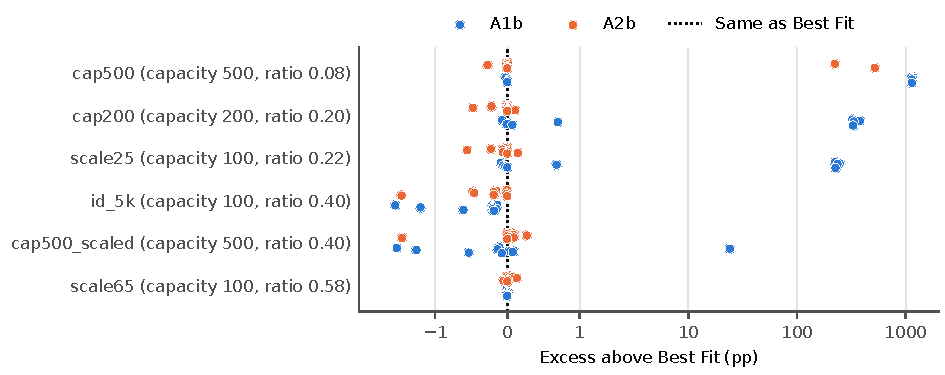
\includegraphics[width=\figwide]{figures/collapses.pdf}
\caption{Excess above Best Fit on each of the six test sets that change item size relative to capacity, with one point per seed; sets are ordered by mean item size relative to capacity (ratio). Points on the dotted line match Best Fit, and a seed collapses if it lies more than 100\,pp to the right. A1b trains at ratio 0.40, and A2b at ratios 0.13 and 0.40. The horizontal axis is symmetric-logarithmic.}
\label{fig:ratio}
\end{figure*}

\paragraph{Mixed capacities (A2b).} No seed collapses on \texttt{cap200} or \texttt{scale25} (4 of 10 each in A1b, $p=0.087$), and two do on \texttt{cap500} (5 of 10, $p=0.35$). In A1b, the collapsing seeds lie 1,138--1,142\,pp above Best Fit on \texttt{cap500}, 324--378\,pp on \texttt{cap200} and 225--247\,pp on \texttt{scale25}, and the two collapsing A2b seeds lie 222 and 520\,pp above it on \texttt{cap500}. No seed of either setting collapses on \texttt{cap500\_scaled}, where the largest loss is 24\,pp. Neither reduction in collapses is significant. Seeds worse than Best Fit on \texttt{scale25} fall from 5 of 10 to 0 ($p=0.033$, one of several uncorrected comparisons with A1b), one more than the collapse count because A1b seed 4 loses 0.68\,pp there without collapsing. The pattern is consistent with the ratio explanation (Figure~\ref{fig:ratio}): training at ratios 0.13 and 0.40 removes collapses at 0.20--0.22, within that range, and reduces them from 5 seeds to 2 at 0.08, outside it. The cost in distribution is modest, a mean gain of 0.35\,pp against A1b's 0.56\,pp. Rescored on A2b's training set, A1b's collapsing programs reach 122--324\% excess against Best Fit's 2.96\%, so selection under mixed capacities would have rejected them. Five of ten programs still read the largest bin, which suggests that varied training selected against fragile rules without preventing rules from reading the capacity. Validation did not detect this failure: it selects seed 8, which is 520\,pp above Best Fit on \texttt{cap500}, because the validation instances share the training ratio. A2b's remaining collapses are confined to its two fresh-bin seeds, 2 and 8, and seed 8 is also 29\,pp worse than Best Fit on \texttt{shape\_k5}.

\subsection{Testing the explanations}
\label{sec:res-tests}
Stages~1--3 suggest explanations but do not establish them, so Stage~4 tests them with three checks that require no further search (Table~\ref{tab:attribution}).

First, we withhold empty bins by re-scoring under AnyFit. No AnyFit rule can exceed about twice the lower bound, so the disappearance of collapses is expected. The informative result is that the withheld rules land within 0.03\,pp of Best Fit on the sets where they had collapsed. Withholding also changes what a capacity-reading rule sees as the largest bin, so, second, we keep empty bins visible to the rule but do not allow them to be chosen while a used bin fits. A1b seeds 0, 2, 3 and 9 then match Best Fit to two decimal places on \texttt{id\_5k}, \texttt{cap200}, \texttt{cap500} and \texttt{scale25}: their only departure from Best Fit is when they open an empty bin. Retained gains depend on the check, as A1b seed 4 keeps 0.81\,pp on \texttt{id\_5k} under this masked choice but loses 0.21\,pp under AnyFit.

Third, we construct a case where the rules should fail, by lowering the item-to-bin ratio. A1b seed 0 scores a used bin $-(1+g/C)^3$ and an empty bin the constant $-2.5$, so an empty bin wins whenever a used one would be left with more than 36\% of its capacity. A bin holding one item of relative size $\rho$ is left with $1-2\rho$ after a second, which predicts that failure begins below $\rho\approx0.32$. We derived this prediction from seed 0's constants alone, not from the sweep, and tested it on new instances at capacity 100 (five instances of 2,000 items per ratio; Figure~\ref{fig:sweep}). Seed 0 is 0.3\,pp better than Best Fit at $\rho=0.36$ and then 4.7\,pp worse at 0.31, 67\,pp at 0.27 and 201\,pp at 0.23, so failure begins where predicted and reaches our 100\,pp definition of collapse between 0.27 and 0.23; seeds 2, 3 and 9 follow the same pattern, and seed 4 fails only at smaller ratios (18\,pp at 0.18, 290\,pp at 0.13). Holding the ratio at 0.40 and raising the capacity to 1,000 causes no collapse in any of the five rules, although seed 2 loses 42\,pp because it also has an absolute gap term. The sweep was designed after scoring and is exploratory, but for these five rules it supports the ratio explanation directly.

\begin{figure}[t]% onecolumn
\centering
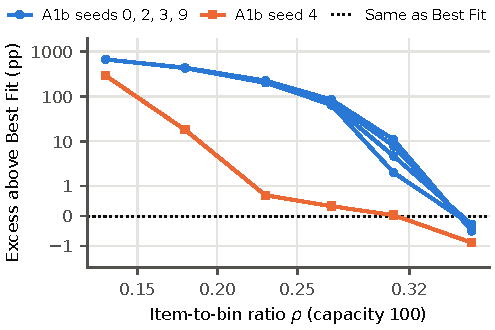
\includegraphics[width=\figw]{figures/ratio_sweep.pdf}
\caption{Excess above Best Fit of the five A1b rules that collapse on \texttt{cap500}, on new instances at capacity 100 as the item-to-bin ratio $\rho$ is varied. Training is at $\rho=0.40$, and seed 0's constants predict failure below $\rho\approx0.32$. The vertical axis is symmetric-logarithmic. Exploratory.}
\label{fig:sweep}
\end{figure}

\begin{table*}[t]
\centering\footnotesize
\caption{Attribution of each observed failure. Excess (\%) is shown as offered empty bins $\rightarrow$ not offered.}
\label{tab:attribution}
\begin{tabularx}{\linewidth}{@{}p{0.2\linewidth}lp{0.22\linewidth}X@{}}
\toprule
Failure & Rules & Evidence & Mechanism\\
\midrule
Loss on \texttt{shape\_k5} & Baseline 4, 5; tuned & $10.81\rightarrow 8.19$; $30.36\rightarrow 8.25$ & Fresh-bin strategy on clustered sizes\\
Loss on \texttt{shape\_k1.5} & Baseline 3 & $3.90\rightarrow 3.99$ & Not fresh bins: underflow reduces the rule to First Fit with a window of avoided bins\\
Collapse at small ratios & A1b 0, 2, 3, 4, 9 & \texttt{cap500}: $1142\rightarrow 0.5$ & Empty-bin score on a scale fitted to the training ratio (seeds 0, 2, 3, 4, 9; seed 2 also has an absolute gap term), with capacity read from the largest bin\\
Collapse outside the trained range & A2b 2, 8 & \texttt{cap500}: $223$, $520\rightarrow 0.5$ & Multiplicative empty-bin penalty (seed 2) and fill-ratio targets (seed 8), neither an empty-bin constant\\
Loss on \texttt{cap500\_scaled} & Tuned & 5.19, and 5.20 tuned under AnyFit & Gap thresholds in absolute item units\\
\bottomrule
\end{tabularx}
\end{table*}

\subsection{Cost of discovery and cost of use}
\label{sec:res-cost}
\begin{table*}[t]
\centering\footnotesize
\caption{Discovery and use costs, means per run. ``Unique'' counts distinct programs of 300, ``Median best eval'' is when the final rule was found, and ``Time'' is per \texttt{id\_5k} instance and was not measured under controlled conditions. The last three columns give the seed with the lowest mean validation excess and the number of the eleven test sets on which it is better/worse.}
\label{tab:cost}
\setlength{\tabcolsep}{4pt}\begin{tabular}{@{}lrrrrrrrrr@{}}
\toprule
Setting & \$/run & Tokens/run & Valid \% & Unique & Median best eval & Time (s) & Selected seed & vs Best Fit & vs tuned\\
\midrule
Baseline & 0.17 & 201k & 99.1 & 207 & 180 & 0.74 & 4 & 6/0/4/1 & 4/0/3/4\\
A1a & 0.18 & 211k & 99.3 & 208 & 226 & 0.32 & 1 & 9/0/1/1 & 6/0/5/0\\
A1b & 0.23 & 267k & 98.9 & 257 & 217 & 2.13 & 1 & 8/0/3/0 & 5/0/4/2\\
Control & 0.09 & 111k & 99.6 & 30 & 1 & 0.45 & 0 & 0/11/0/0 & 4/0/3/4\\
A2a & 0.17 & 202k & 99.3 & 222 & 154 & 0.99 & 6 & 8/0/2/1 & 6/0/4/1\\
A2b & 0.22 & 267k & 99.0 & 250 & 160 & 1.19 & 8 & 3/0/4/4 & 3/0/1/7\\
\bottomrule
\end{tabular}

\end{table*}

Discovery is inexpensive: a run costs \$0.17--0.23 with EoH, including unsuccessful proposals and evaluations, and \$0.09 with the control, and tuned Best Fit needs no LLM (Table~\ref{tab:cost}). In EoH the final rule typically appears after 150--230 evaluations, so most of the 300 are used. All final programs completed every instance, so the Next Fit fallback was never applied, and every best program passed the integrity checks, unchanged under repeated and shuffled scoring. Evolved rules take 0.3--2.1\,s per \texttt{id\_5k} instance and tuned Best Fit, scored the same way, 0.2--1.4\,s (\texttt{final\_per\_instance.csv} in each setting's results folder). These times were not measured under one controlled load and indicate only the order of magnitude. Best Fit's 0.03\,s comes from a dedicated packer outside this path and is not comparable.

\section{Discussion and limitations}
Two results temper the usual reading of comparisons between evolved rules and Best Fit. Beating Best Fit is not evidence of the LLM's contribution here, because a three-parameter tuner under the same budget beats it by more, and only 1 of 50 evolved rules beat the tuner of its own setting in distribution. The tuner wins there because its form, taken from FunSearch, already encodes the fresh-bin strategy, so random search reaches most of its gain within about 10 evaluations (Figure~\ref{fig:convergence}), whereas EoH must discover the strategy and its median stays at Best Fit's level until evaluation 186. Nor should the evolved rules' better behaviour under shift be read as an inherent strength, since tuned Best Fit's largest loss disappears once it is trained on mixed shapes, at the price of losses elsewhere. Evolution mattered at this budget: without it, all ten RandSample seeds stayed at Best Fit, although the control's different prompt means search and prompt cannot be separated. An informed prompt made in-distribution gains over Best Fit reliable, as all ten seeds beat it, but none beat the tuner. The same prompt preceded the worst failures, which suggests that additional information can enlarge the ways in which search fits the training set. A1b changes the task framing and the bin description together, so we cannot conclude which element is responsible.

In these runs, the largest gains and the worst failures were associated with two behaviours, supported by re-scoring the programs, reading their code and sweeping the ratio. The first is whether a rule opens empty bins while a used bin could hold the item. This strategy carries the largest gains we observed, for evolved rules and for tuning alike, and its outcome on clustered sizes tracks how often it is used (Figure~\ref{fig:phi}). The second is whether a rule's constants are tied to the training item-to-bin ratio, which accounts for most collapses of informed rules. Two further mechanisms, numerical underflow and absolute gap thresholds, explain the remaining failures (Table~\ref{tab:attribution}). Training data affects which of these failures survive selection. Mixed shapes removed tuned Best Fit's large loss on \texttt{shape\_k5}, with no overlap between seeds (27.7--35.2\% against 6.9--9.8\%), although it introduced losses on \texttt{scale25} and \texttt{shape\_k1.5}, whereas A2b's reduction in the evolved rules' collapses is consistent with an effect but not significant, and it may reflect selection against fragile rules and not rules that adapt (Section~\ref{sec:a2}). Both behaviours exploit a regularity that the training set holds fixed, the spread of item sizes or the item-to-bin ratio, which is why varying it in training removed some failures and why validation drawn from the training distribution missed them.

Several limitations follow from the design. We use one inexpensive model and one search method at 300 evaluations per run, so our conclusions concern this regime, and equal evaluations are not equal distinct candidates, since up to about a third of EoH's are repeats. Our setup differs from EoH's in several ways at once (Table~\ref{tab:eoh}), so differences from its reported gains have no single cause. A2b is conditional on the informed prompt. Tuned Best Fit's form draws on prior knowledge not charged to its budget, and its absolute parameters are not adapted to capacity. Ten seeds leave most setting-level differences non-significant, including A2b's reduction in collapses, so those results rest on the consistency of the pattern. Our explanations rest on re-scoring and on reading selected programs, not on editing every rule, and the role of the item-to-bin ratio was identified after scoring and tested by sweep for only five rules.

\section{Conclusion}
In these experiments, the largest gains and most failures of evolved rules were associated with two behaviours: opening an empty bin while a used bin has room, and constants fitted to the training item-to-bin ratio. With 300 evaluations and an inexpensive model, evolved rules matched or modestly improved on Best Fit in distribution, but they almost never outperformed a three-parameter tuned variant there. Two effects held in every seed: without evolution, under RandSample's prompt, the LLM never passed Best Fit, and stating the task and bin rules made every seed beat it. Validation drawn from the training distribution did not reveal the failures, so validation should vary the item-to-bin ratio. Varied training moved tuned Best Fit's failure to other sets, and it reduced evolved rules' collapses on all three sets where A1b collapsed (from 4, 4 and 5 of 10 seeds to 0, 0 and 2), although not significantly. It remains open whether a larger budget or a stronger model would change the comparison with tuning, and whether ratio-dependence can be prevented during search.

\paragraph{Reproducibility.} The repository contains all configurations, instance definitions, every evaluated program, scores, LLM logs and saved results. Scoring, statistics, the checks of Section~\ref{sec:res-tests} (\texttt{masked\_choice.py}, \texttt{ratio\_sweep.py}), tables and figures are regenerated without LLM calls by the commands given in its readme, and \texttt{verify\_report\_numbers.py} checks every number quoted in this report against the committed results. Design decisions, failed attempts and corrections are logged in \texttt{code/docs/log.md}.

{\footnotesize
\bibliographystyle{alpha}
\bibliography{references}
}

\end{document}
